\documentclass[11pt]{beamer}
\usetheme[progressbar=frametitle]{metropolis}
\usepackage{xcolor} %Farbe überschriften
\definecolor{blue}{RGB}{24,116,190}
\setbeamercolor{progress bar}{fg=blue}

%\usecolortheme{owl}

\usepackage{appendixnumberbeamer}
\usepackage[utf8]{inputenc}
\usepackage[T1]{fontenc}
\usepackage{graphicx}
\usepackage{lmodern}
%\usepackage{beamercolorthemeowl}
\usepackage{pgfpages}
%\setbeameroption{show notes} %Notizen anzeigen
%\setbeameroption{show notes on second screen}
\makeatletter
\setlength{\metropolis@progressinheadfoot@linewidth}{3pt}
\setlength{\metropolis@titleseparator@linewidth}{1pt}
\setlength{\metropolis@progressonsectionpage@linewidth}{3pt}

\author{Laura Hartzheim}

\title{Arten des Machine Learnings - Supervised, Unsupervised und Reinforcement Learning}

\subtitle{}

\logo{}

\institute{}

\date{}

\subject{}

\setbeamercovered{transparent}

\setbeamertemplate{navigation symbols}{}

\begin{document}
	
	
	\begin{frame}
		\titlepage
	\end{frame} 
	
	\begin{frame}
		\frametitle{Inhalt}
		\tableofcontents
	\end{frame} 
	
	\section{Machine Learning}
	\begin{frame}
		\frametitle{Was ist Machine Learning?}
		\begin{itemize}
			\item Schnittmenge aus Statistik, Künstlicher Intelligenz und Informatik
			\item Maschine soll aus Daten lernen können, durch Erfahrung und Leistungsmessung
			%Bsp spam filter
		\end{itemize} 
	\end{frame}
	
	\begin{frame}
		\frametitle{Warum nutzt man Machine Learning?}
		\begin{itemize}
			\item vereinfachter Code und bessere Performanz bei Problemen mit vielen Regeln, da Regeln von Machine gelernt werden 
			\item Programme leichter zu warten und weniger fehleranfällig
			\item bietet Lösungen für komplexe Probleme die durch normale Programme nicht lösbar sind
			\item und vieles mehr
			%Email bsp
			
		\end{itemize} 
	\end{frame}
	
	\section{Supervised Learning}
	
	\begin{frame}
		\frametitle{Supervised Learning}
		\begin{itemize}
			\item Nutzen von bekannten Daten und Ausgaben(Label) während des Trainings 
			\item Ziel: eingehende Daten den entsprechenden ausgehenden Daten zuzuordnen
			% Over und Underfitting ?
		\end{itemize}
	\end{frame}
	
	\begin{frame}
		\frametitle{Klassifikation}
		\begin{itemize}
			\item Ziel: Klassenlabel für die eingehenden Daten voraussagen
			\item binäre Klassifikation: nur zwei mögliche Label $\rightarrow$ Ja/Nein-Frage
			\item multiklassen Klassifikation: mehrere Klassen möglich
			\item Erstellen von Regeln während der Trainings-Phase 
		\end{itemize}
		
	\end{frame}
	
	\begin{frame}
		\frametitle{Klassifikation}
		\centering
		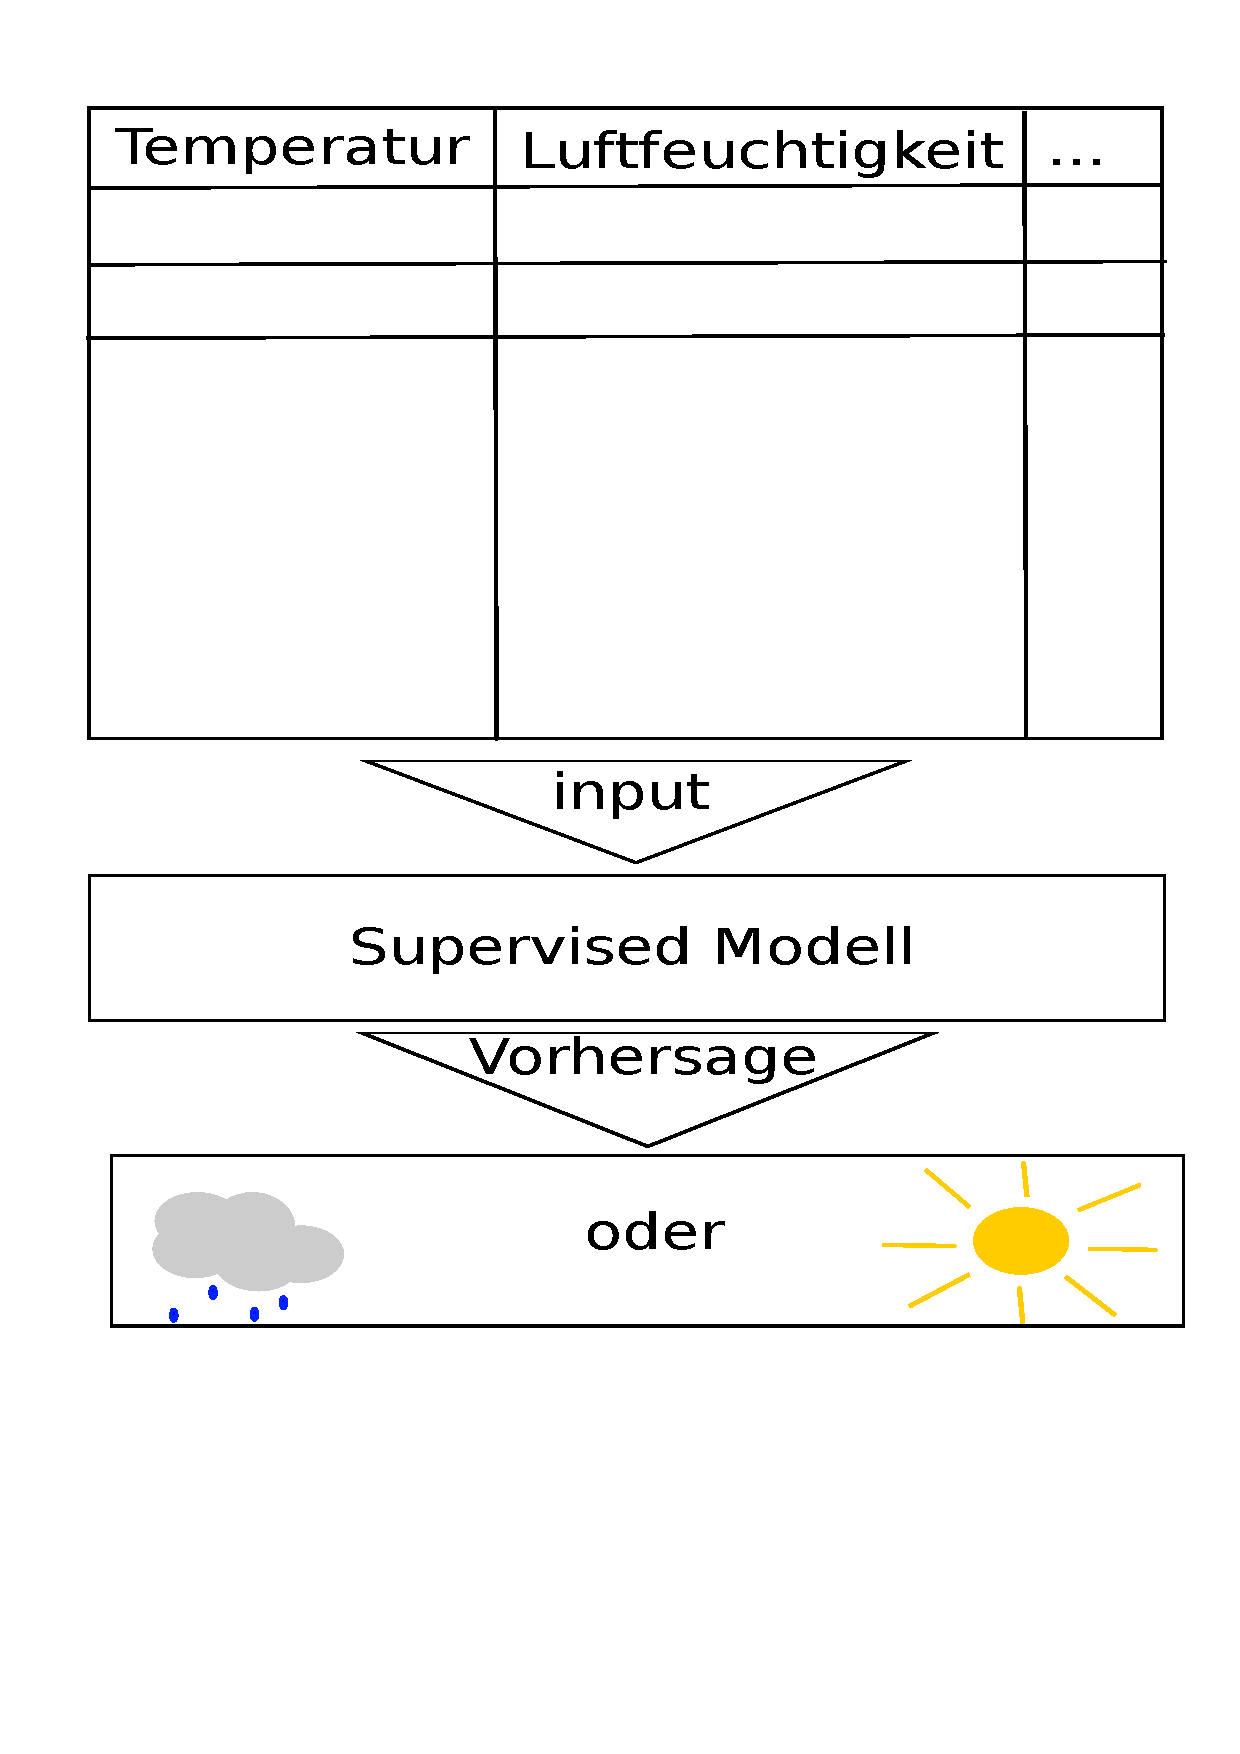
\includegraphics[width=200pt]{C:/Users/Laura/Documents/GitHub/LaTexSeminar/bilder/Label.pdf}
	\end{frame}
	
	\begin{frame}
		\frametitle{Regression}
		\begin{itemize}
			\item Ziel: Ermitteln von Werten
			\item keine Klassen
			\item lernen der Zusammenhangs der In- und Output Daten
			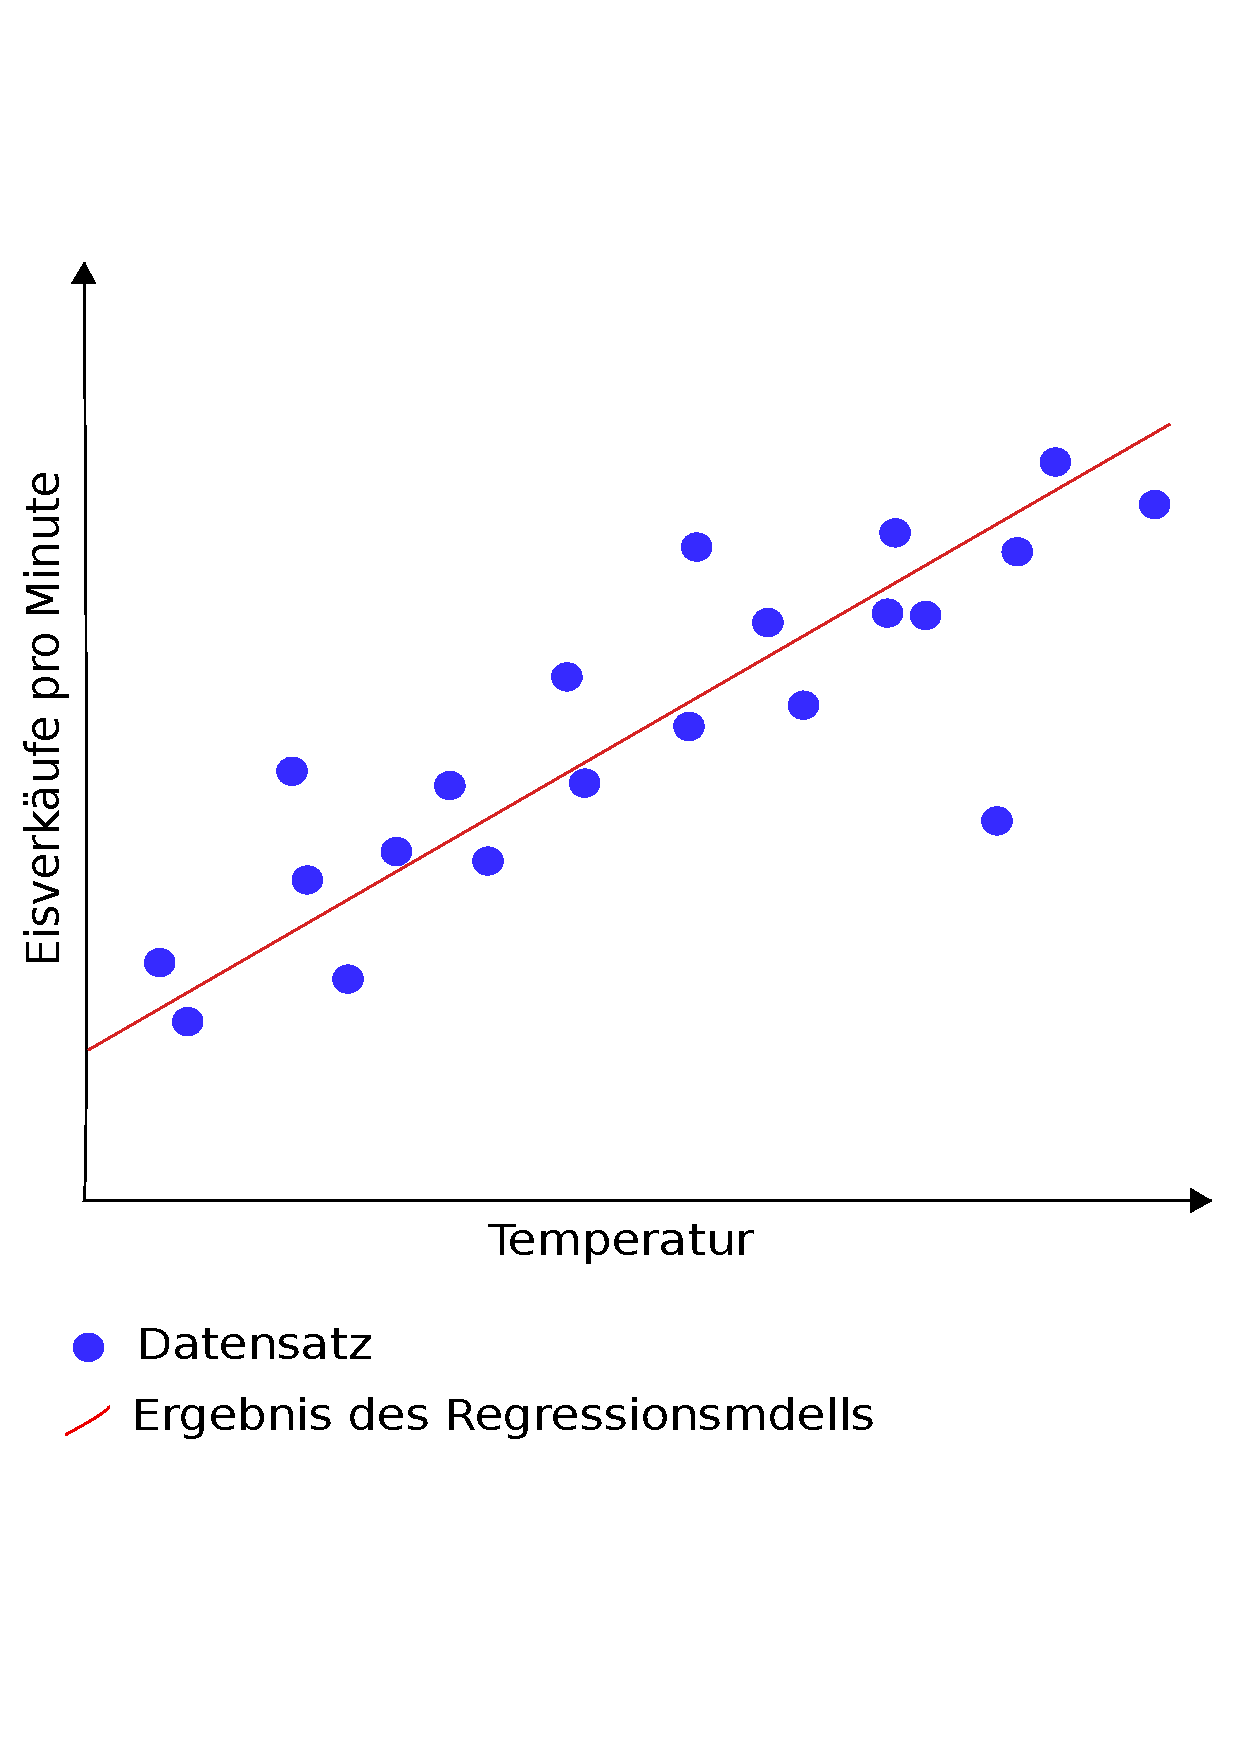
\includegraphics[width=200pt]{C:/Users/Laura/Documents/GitHub/LaTexSeminar/bilder/Regression.pdf}
		\end{itemize}
		
	\end{frame}
	
	\section{Unsupervised Learning}
	
	\begin{frame}
		\frametitle{Unsupervised Learning}
		\begin{itemize}
			\item keine bekannten Output-Daten/Label beim Training
			\item schwer feststellbar ob Modell korrekte Ergebnisse erzielt
			\item Maschine bekommt Input-Daten und muss anhand dieser Entscheidungen treffen und kategorisieren
			\item Modell lernt Muster, Strukturen und Beziehungen in Datensätzen
		\end{itemize}
	\end{frame}
	
	\begin{frame}
		\frametitle{Clusterbildung}
		\begin{itemize}
			\item Ziel: in jedem Cluster möglichst ähnliche Daten, die sich zu Daten aus anderen Clustern unterscheiden
			\item Clusterbildung durch Muster, Ähnlichkeiten und Verbindungen zwischen Datensätzen
		\end{itemize}
		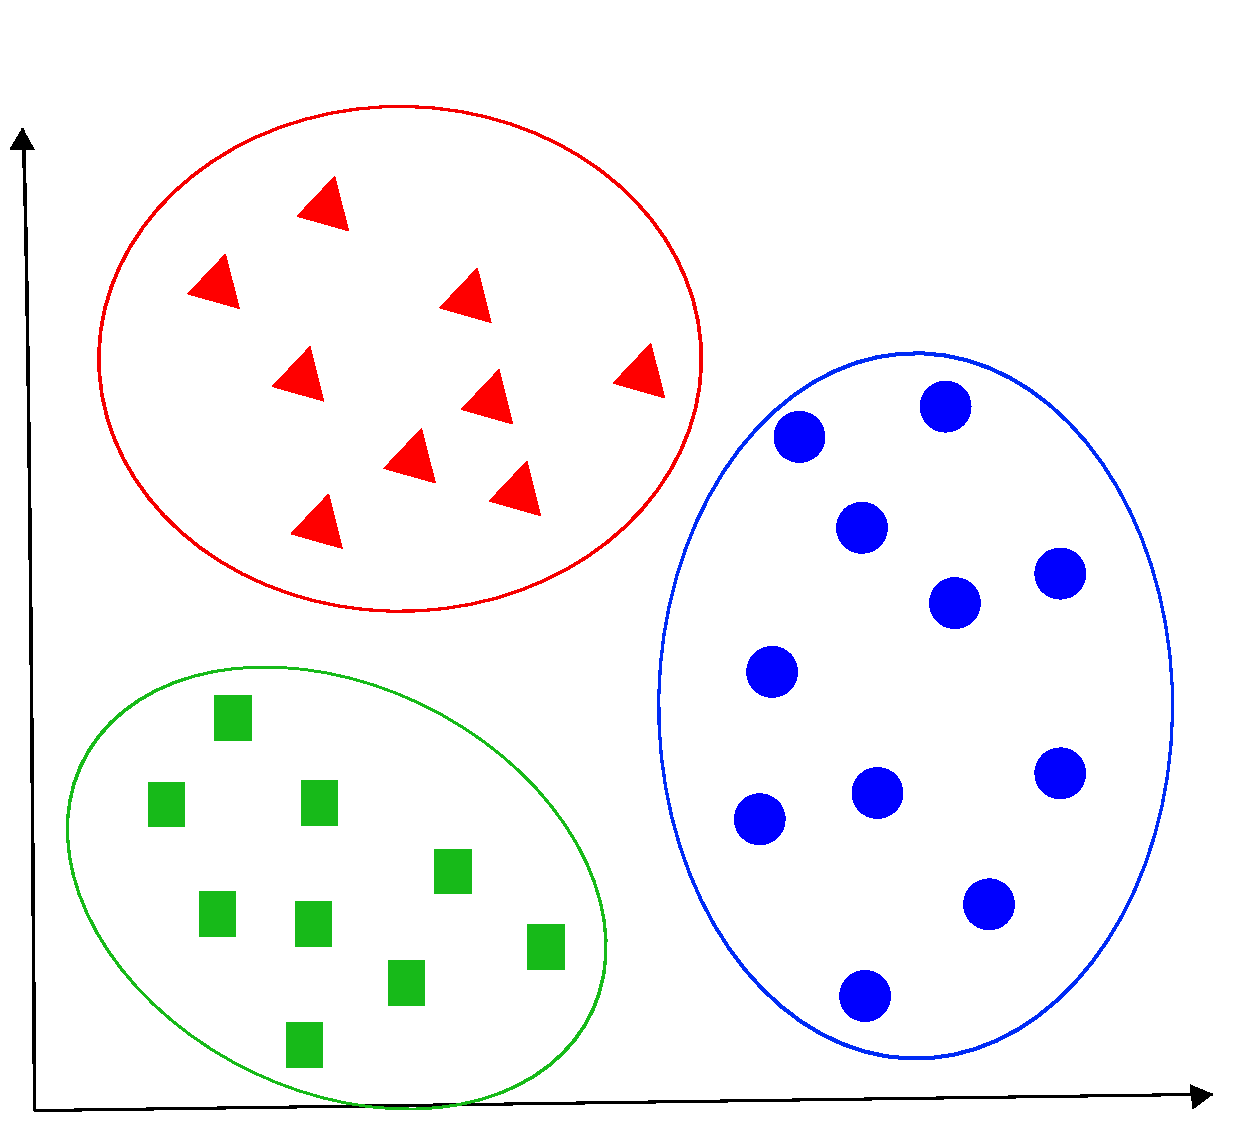
\includegraphics[width=130pt]{C:/Users/Laura/Documents/GitHub/LaTexSeminar/bilder/Cluster.pdf}
	\end{frame}
	
	\begin{frame}
		\frametitle{Dimensionsreduktion}
		\begin{itemize}
			\item 
		\end{itemize}
		Die Komplexität des Machine Learning Modells ist abhängig von der Anzahl der Inputs. Sie bestimmen die Zeit- und Speicherkomplexität, sowie die Anzahl der zum Training benötigten Daten. [6] Dimensionsreduktion wird genutzt um den überladenen InputSpace zu verkleinern. Somit wird die Anzahl der relevanten Features oder Attribute(b = Dimensionen) für jeden Datensatz reduziert. [4] Wenn die Modelle einfach gehalten werden, sind sie, aufgrund ihrer geringeren Varianz, bei kleinen Datensätzen robuster. [6] Die Reduktion der Dimensionen erfolgt durch die Auswahl von Hauptfeatures und bedarfsgesteuerten Features. Für diese gibt es zwei Methoden. [4] Für die Feature Extraction werden neue Features, die Kombinationen aus der origni
		7
		nalen Featureliste sind, gesucht. [6] Bei der Feature Selection werden von d Dimensionen k, mit Hilfe von Subset Selection, ausgewählt. [6] Die Features, die die meisten Informationen liefern, werden aus der originalen Featureliste ausgewählt, der Rest wird verworfen. Es kommen keine neuen Features hinzu. [4] Ziel der Subset Selection ist es, das beste Subset aus der Featureliste mit einer möglichst geringen Anzahl von Dimensionen und der besten Genauigkeit zu nden. Es gibt 2d mögliche Subsets aus denen ausgewählt werden kann. Aufgrund der groÿen Menge können nicht alle getestet werden, deswegen müssen geeignete Verfahren für die Auswahl genutzt werden. [6]
		
	\end{frame}
	
	\begin{frame}
		\frametitle{}
		\begin{itemize}
			\item 
		\end{itemize}
	\end{frame}
	
	\section{Reinforcement Learning}
	
	\begin{frame}
		
	\end{frame}
	

\end{document}